\clearpage
% ==========================
\section{Grundlagen}
% ==========================

% ==========================
\subsection{Raspberry Pi}
Ein Raspberry Pi ist ein kompakter, kostengünstiger Einplatinencomputer, der ursprünglich von der Raspberry Pi Foundation entwickelt wurde. Dank seiner kompakten Bauweise und seines erschwinglichen Preises ist der Raspberry Pi ein vielseitiges und leistungsfähiges Werkzeug, welches von kleineren Projekten bis hin zu anspruchsvollen industriellen Anwendungen eingesetzt wird.
%%%%%%%%%%%%%%%%%%%%%%%%%%%%%%%%%%%%%%%%%%%%%%%%%%%%%%%%%%%%%%%%%%%%%%%%%%%
\newline 
\newline 
Hauptmerkmale:
\begin{enumerate}
    \item Kompakte Größe:
    \newline Der Raspberry Pi ist etwa so groß wie eine Kreditkarte, was ihn besonders mobil und platzsparend macht.
    \item Vielseitigkeit:
    \newline Er unterstützt eine Vielzahl von Betriebssystemen (z. B. Raspberry Pi OS, Ubuntu) und kann für Aufgaben wie Programmierung, Netzwerkadministration, Steuerung von IoT-Geräten und Multimedia-Anwendungen verwendet werden.
    \item Erschwinglichkeit:
    \newline Mit einem Preis zwischen 12 € (Raspberry Pi Zero) und etwa 100 € (für High-End-Modelle) ist er eine budgetfreundliche Lösung für Projekte.
    \item Community und Support:
    \newline Der Raspberry Pi hat eine große, aktive Community, die zahlreiche Tutorials, Foren und Open-Source-Projekte bereitstellt.
\end{enumerate}
%%%%%%%%%%%%%%%%%%%%%%%%%%%%%%%%%%%%%%%%%%%%%%%%%%%%%%%%%%%%%%%%%%%%%%%%
Hardwareeigenschaften:
\begin{enumerate}
    \item Prozessor und Arbeitsspeicher:
    \begin{itemize}
        \item Der Raspberry Pi verwendet ARM-basierte Prozessoren, die je nach Modell eine unterschiedliche Leistung bieten.
        \item Die RAM-Größen variieren von 512 MB bis zu 16 GB, je nach Modell.
    \end{itemize}
    \item Anschlüsse und Schnittstellen:
     \begin{itemize}
        \item USB-Ports: Für Maus, Tastatur oder externe Geräte.
        \item HDMI-Ausgang: Für die Bildausgabe auf Monitoren oder Fernsehern.
        \item Ethernet: Für kabelgebundene Netzwerke
        \item Wi-Fi und Bluetooth: Für drahtlose Verbindungen.
        \item GPIO-Pins (General Purpose Input/Output): Ermöglichen die Steuerung und Interaktion mit elektronischen Komponenten wie LEDs und Sensoren.
    \end{itemize}
    \item Speicher:
    \newline Anstelle eines internen Speichers verwendet der Raspberry Pi SD-Karten oder MicroSD-Karten für das Betriebssystem und die Daten.
    \item Energieversorgung:
    \newline Es gibt verschiedene Möglichkeiten einen Raspberry Pi mit Strom zu versorgen:
    \begin{itemize}
        \item USB Power Bank
        \item Batterien/Akkus (AA, 9V, Alkaline, Nickel-Metallhydrid-Akkumulator (NiMH))
        \item USB Kabel am PC/Laptop
    \end{itemize}    
\end{enumerate}



\newpage

% ==========================
\subsubsection{Access Point}
Ein Access Point ist ein Gerät, das als Schnittstelle zwischen kabelgebundenen Netzwerken (z. B. einem Router) und drahtlosen Geräten dient. Er ermöglicht es drahtlosen Geräten wie Smartphones, Laptops oder IoT-Geräten, eine Verbindung zum Netzwerk herzustellen. 
\newline 
\newline 
Hauptfunktionen eines Access Points:
\begin{itemize}
    \item Bereitstellung eines drahtlosen Netzwerks (WLAN):
    \newline Der Access Point erstellt ein lokales WLAN, zu dem sich Geräte verbinden können. Das Netzwerk wird durch die SSID (Service Set Identifier, der WLAN-Name) und eine Verschlüsselung gekennzeichnet.
    \item Verbindung mit kabelgebundenen Netzwerken:
    \newline Der Access Point ist normalerweise mit einem Router, Switch oder Server über ein Ethernet-Kabel verbunden. So verbindet er die drahtlosen Geräte mit dem bestehenden Netzwerk.
    \item Netzwerksicherheit:
    \newline Der Access Point bietet Sicherheitsprotokolle zur Verschlüsselung der Daten.
\end{itemize}
%%%%%%%%%%%%%%%%%%%%%%%%%%%%%%%%%%%%%%%%%%%%%%%%%%%%%%%%%%%%%%%%%%%%%%%%%%%
Es gibt verschiedene Anwendungsbereiche:
\begin{itemize}
    \item Erweitern von Netzwerken:
    \newline Ein Access Point wird oftmals eingesetzt, um die Reichweite eines drahtlosen Netzwerks (z.B. in Büros, Gebäuden oder Fabriken) zu erweitern.
    \item Erstellung lokaler Netwerke
    \newline In  speziellen Anwendungen, wie bei Industrieanlagen, wird ein lokales WLAN-Netzwerk bereitgestellt, ohne dass eine Verbindung zum Internet notwendig ist. Dies ermöglicht eine direkte Kommunikation zwischen Geräten.
    \item Mobile Anwendung:
    \newline Geräte wie Raspberry Pis können als Access Point konfiguriert werden, um ein drahtloses Netzwerk für andere Geräte zu erstellen. Das ist besonders nützlich in Projekten, in denen kein externer Router vorhanden ist.
\end{itemize}
%%%%%%%%%%%%%%%%%%%%%%%%%%%%%%%%%%%%%%%%%%%%%%%%%%%%%%%%%%%%%%%%%%%%%%%%%%%
Funktionsweise eines Access Points:
\newline 
Ein Access Point arbeitet mit den Standards des IEEE 802.11-Protokolls, welche den Betrieb von WLAN-Netzwerken regeln.
\begin{itemize}
    \item Senden und Empfangen von Daten:
    \begin{itemize}
    \item Drahtlose Geräte kommunizieren mit dem Access Point über Funk.
    \item Der Access Point sendet die empfangenen Daten an das kabelgebundene Netzwerk oder an andere Geräte im WLAN weiter. 
    \end{itemize}
   \item Netzwerkverbindung:
   \begin{itemize}
    \item Der Access Point verwendet Ethernet für die Verbindung mit dem Hauptnetzwerk.
    \item Geräte im WLAN erhalten durch den Access Point Zugriff auf Internet oder lokale Ressourcen.
    \end{itemize}
\end{itemize}
%%%%%%%%%%%%%%%%%%%%%%%%%%%%%%%%%%%%%%%%%%%%%%%%%%%%%%%%%%%%%%%%%%%%%%%%%%%
Access Points besitzen verschiedene Vorteile:
\begin{itemize}
    \item Drahtlose Verbindung: Keine Kabel erforderlich, um Geräte zu verbinden.
    \item Flexibilität: Geräte können sich frei im Bereich des WLANs bewegen.
    \item Skalierbarkeit: Mehrere Access Points können kombiniert werden, um größere Netzwerke zu realisieren.
    \item Isolierte Netzwerke: Für spezifische Anwendungen kann ein eigenständiges, lokales Netzwerk eingerichtet werden, das völlig unabhängig vom Internet arbeitet. 
\end{itemize}





% ==========================
\subsection{Standard OPC UA}
% ==========================

Merkmale von OPC UA:
\begin{itemize}
    \item Plattformunabhängigkeit: 
    \newline OPC UA ist nicht an ein bestimmtes Betriebssystem oder eine bestimmte Programmiersprache gebunden. Dies ermöglicht die Implementierung auf unterschiedlichsten Plattformen, von kleinen eingebetteten Systemen bis hin zu großen Industrie-PCs.
    \item Integration von Daten und Metadaten: 
    \newline OPC UA ermöglicht den Austausch von Daten, wie z. B. Sensorwerten oder Maschinendaten, und bietet gleichzeitig Zugriff auf zusätzliche Infos wie Einheiten, Zeitstempel oder Zugriffsrechte.
    \item  Skalierbarkeit: 
    \newline Der Standard ist flexibel und kann sowohl in kleinen Geräten wie einem Sensor als auch in komplexen Produktionsanlagen eingesetzt werden.
    \item Sicherheit:
    \newline OPC UA bietet integrierte Sicherheitsmechanismen wie Authentifizierung, Datenverschlüsselung, und Datenintegrität.
    \item Interoperabilität:
    \newline OPC UA ermöglicht die Kommunikation zwischen Geräten und Systemen unterschiedlicher Hersteller.  
    \item Modellierung komplexer Datenstrukturen:
    \newline OPC UA unterstützt die Abbildung komplexer Datenmodelle, sodass Maschinen- und Prozessdaten in einer strukturierten Form bereitgestellt werden können.
\end{itemize}
Wir haben uns für das MQTT-Protokoll entschieden, welches folgende Vorteile bietet:
\begin{enumerate}
    \item Zuverlässigkeit: MQTT bietet verschiedene Quality of Service (QoS)-Level, die sicherstellen, dass Nachrichten korrekt übertragen werden.
    \item Echtzeitfähigkeit: Daten werden nahezu in Echtzeit zwischen den Geräten ausgetauscht. Die Echtzeitfähigkeit ist für unser Projekt essenziell.
    \item Flexibilität: Die Topics können flexibel strukturiert werden, sodass mehrere Datenarten gleichzeitig verarbeitet werden können.
    \item Leichtgewichtig: Das Protokoll benötigt nur minimale Ressourcen wie Rechenleistung, Speicher und Bandbreite, was es ideal für Geräte wie den Raspberry Pi macht.
\end{enumerate}


 
\clearpage
% ==========================
\subsection{Android App}
% ==========================
Die Programmierung der App wird mit dem Programm \texttt{Android Studio Ladybug} in der Version \texttt{2024.2.1 Patch 2} verwendet. Als Programmiersprache wird Kotlin gewählt, da diese sich besonders gut für die Entwicklung einer Android App eignet.
\\
\noindent In einer Android App wird alles in \glqq Aktivitäten\grqq organisiert. Dabei kann man sich eine Aktivität wie ein Bildschirm in der App vorstellen. Beispielsweise ist die Startseite eine Aktivität und der Bildschirm, der die MQTT Daten anzeigt eine andere Aktivität.
Jede Aktivität ist gleich aufgebaut und hat einen festen Lebenszyklus, der aus folgenden Komponenten besteht. Diese sind auch in \autoref{fig:AndroidLifecycle} dargestellt.
\begin{enumerate}
    \item \textbf{onCreate()}: wird aufgerufen, wenn die Aktivität zum ersten Mal erstellt wird
    \item \textbf{onStart()}: Die Aktivität wird für den Nutzer sichtbar, dieser kann aber noch nicht mit der App interagieren
    \item \textbf{onResume()}: hier ist die App komplett sichtbar und der Nutzer kann interagieren
    \item \textbf{onPause()}: eine andere App wird geöffnet und  diese Aktivität wird pausiert. Sie ist also nicht mehr im Vordergrund
    \item \textbf{onStop()}: die Aktivität wird nicht mehr Benutzt. Es wird zum Beispiel eine andere Aktivität geöffnet. Jedoch wird die Aktivität nicht zerstört
    \item \textbf{onRestart()}: wird neu gestartet, wenn der Nutzer zur Aktivität zurückkehrt
    \item \textbf{onDestroy()}: die Aktivität wird komplett zerstört und vom System entfernt.
\end{enumerate}
Diese Komponenten eignen sich beispielsweise auch sehr gute zum Debuggen. Hier kann überprüft werden in welchem Zustand sich die Aktivität befindet.

\begin{figure}[h!]
    \centering
    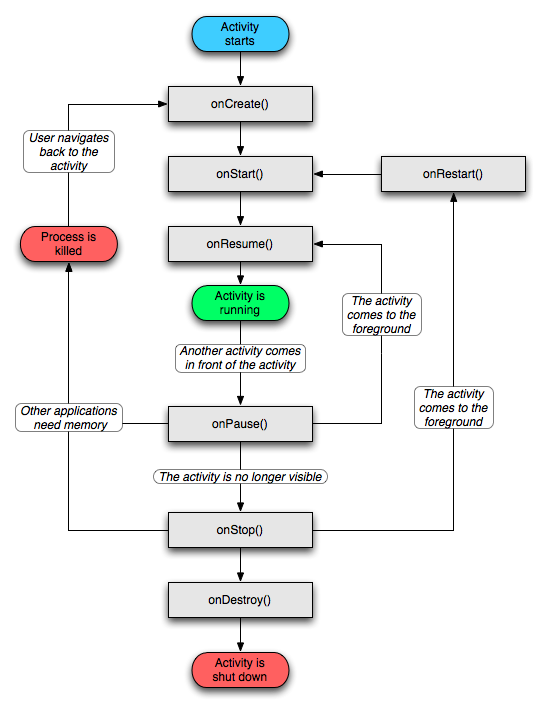
\includegraphics[width=0.5\textwidth]{pictures/AndroidLifecycle.png}
    \caption{Eine vereinfachte Darstellung des Aktivitätslebenszyklus}
    \label{fig:AndroidLifecycle}
\end{figure}
\clearpage